\documentclass[11pt]{article}
\usepackage{latexsym}
\usepackage{amsmath}
\usepackage{amssymb}
\usepackage{amsthm}
\usepackage{epsfig}
\usepackage[hyphens,spaces,obeyspaces]{url}
\usepackage[colorlinks,allcolors=blue]{hyperref}
\usepackage[tight]{subfigure}

\usepackage{amsmath}

\DeclareMathOperator*{\minimize}{min}
\DeclareMathOperator*{\maximize}{max}

\usepackage{algorithm}
 %on linux you may need to run sudo apt-get install texlive-full to install algorithm.sys
\usepackage{algorithmic}

\usepackage{verbatim}
\usepackage{amsmath,amsfonts,amsthm,bm}

\newcommand{\handout}[5]{
  \noindent
  \begin{center}
  \framebox{
    \vbox{
      \hbox to 5.78in { {#1} \hfill #2 }
      \vspace{4mm}
      \hbox to 5.78in { {\Large \hfill #5  \hfill} }
      \vspace{2mm}
      \hbox to 5.78in { {\em #3 \hfill #4} }
    }
  }
  \end{center}
  \vspace*{4mm}
}

\newcommand{\lecture}[5]{\handout{#1}{#2}{#3}{#4}{#5}}
\newcommand{\collision}[0]{\mathrm{collision}}
\newcommand{\nocollision}[0]{\overline{\collision}}

\newcommand*{\QED}{\hfill\ensuremath{\square}}

\newtheorem{theorem}{Theorem}
\newtheorem{corollary}[theorem]{Corollary}
\newtheorem{lemma}[theorem]{Lemma}
\newtheorem{observation}[theorem]{Observation}
\newtheorem{proposition}[theorem]{Proposition}
\newtheorem{definition}[theorem]{Definition}
\newtheorem{claim}[theorem]{Claim}
\newtheorem{fact}[theorem]{Fact}
\newtheorem{assumption}[theorem]{Assumption}
\newtheorem{note}[theorem]{Note}

% 1-inch margins, from fullpage.sty by H.Partl, Version 2, Dec. 15, 1988.
\topmargin 0pt
\advance \topmargin by -\headheight
\advance \topmargin by -\headsep
\textheight 8.9in
\oddsidemargin 0pt
\evensidemargin \oddsidemargin
\marginparwidth 0.5in
\textwidth 6.5in

\parindent 0in
\parskip 1.5ex
%\renewcommand{\baselinestretch}{1.25}

\begin{document}

\lecture{Statistical Techniques in Robotics (16-831, S22)}{Lecture \#13
  (Wednesday, March 02)}{Lecturer: Kris Kitani}{Scribes: Dakshit Agrawal, Meghdeep Jana}{Thompsons Sampling, EXP3, EXP4}

\section{Review}
%This section serves as a review of the previous lecture and any other context required to frame the content of the current lecture. 

%You may format the scribes in any way you like, aside from changing font style, size and page format. Please use subsections and paragraphs to increase the readability of your notes.

%Length requirement 1-2 pages.

In the previous lecture, we discussed two multi-arm bandit(MAB) algorithms: Explore-Exploit and Upper Confidence Bound(UCB). We review these algorithms

\begin{figure}[h]
    \centering
    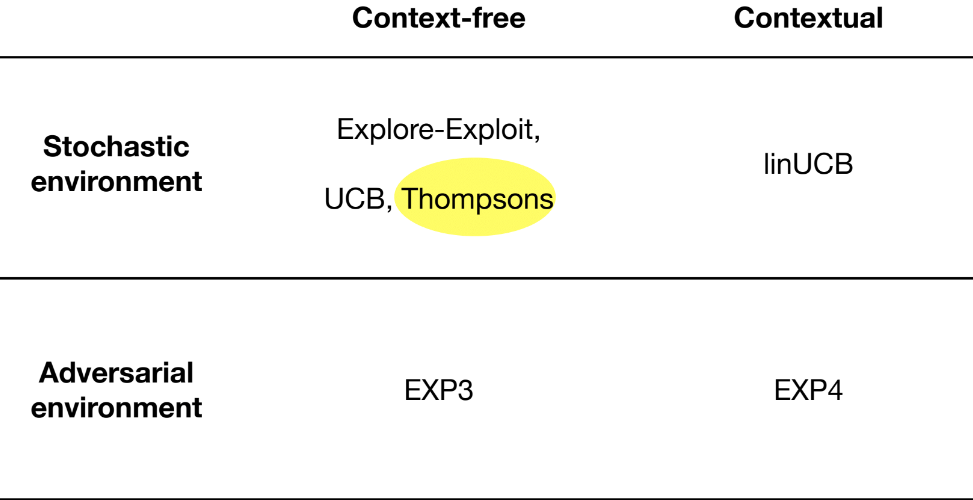
\includegraphics[width=0.5\textwidth]{figs/mab.png}
    \caption{Types of MAB Algorithms}
    \label{fig:mab}
\end{figure}

\subsection{Explore-Exploit}
\label{sec:expexp}
The Explore-Exploit algorithm is shown in Algorithm \ref{algo:exprexpl}.

\begin{algorithm}[H]
\caption{Explore-Exploit\cite{exp2}}
\label{algo:exprexpl}
\begin{algorithmic}[1]
\REQUIRE $M$
\FOR{$k=1,\;\cdots,\;K$}
\FOR{$m=1,\;\cdots,\;M$}
\STATE $a = k$
\STATE $\text{Receive}(r)$
\STATE $\hat{\mu}_k = \hat{\mu}_k + \frac{r}{M}$
\ENDFOR
\ENDFOR
\FOR{$t=KM,\;\cdots,\;T$}
\STATE $a^{(t)} = \arg\max_{k}\widehat{\mu}_k'$
\ENDFOR
\end{algorithmic}
\end{algorithm}

The algorithm has two phases (a) Explore phase(lines 1-7) where we make $KM$ pulls  (b) Exploitation Phase(lines 8-10) where go from round $KM$ to $T$. The regret is derived for each phase using the Hoeffding's inequality. 

\definition{\textbf{Hoeffding's inequality}\normalfont\cite{hoeff}: Consider a one-dimension distribution $\nu$ with expectation $\mu$, where any sample $r \sim \nu$ is bounded such that $r \in [0,1]$. Given $T$ i.i.d. samples ${r^{(t)}}_{t=1}^T$, we have that for any $\epsilon$:
\begin{equation}
    p(|\sum_{t=1}^T \frac{r^{(t)}}{T} - \mu | \geq \epsilon) \leq 2e^{-2T\epsilon^2}
\end{equation}
}
\normalfont

We get the regret bound for explore phase as $R_{\text{explore}} = \mathcal{O}(KM)$ and for the exploit phase, we get $R_{\text{exploit}} = \sum_{t=KM+1}^T (\mu_{k^*}^{(t)} - \mu_{\hat{k}}^{(t)}) \leq (T - KM) \cdot 2 \sqrt{\frac{\log (2/\delta)}{2M}}$. We get the total regret bound by adding the two regrets and upper bounding it.

\begin{equation}
R_{\text{explore-exploit}} \leq KM + 2T \cdot \sqrt{\frac{1}{M}}
\end{equation}


The optimal M was found to be $(\frac{T}{K}^{2/3})$. From this we get the Asymptotic Regret bound as $R_{\text{explore-exploit}}  =  \mathcal{O}(K^{1/3}T^{2/3})$. Which shows that Explore-Exploit grows sublinearly with time and is a no-regret algorithm.

\subsection{UCB}
\label{sec:ucb}
Using the Heoffding's inequality, a confidence bound is defined.
\definition{\textbf{Confidence Bound:} \normalfont We get that the optimal value of $\epsilon$ for which the hoeffding's inequality is upper bounded by a specified value $\delta$ is:
\begin{equation}
    \epsilon = \sqrt{\frac{log(2/\delta)}{2T}}
\end{equation}
}
\normalfont
The UCB algorithm is shown in Algorithm \ref{algo:UCB}.

\begin{algorithm}[H]
\caption{UCB}
\label{algo:UCB}
\begin{algorithmic}[1]
\REQUIRE $\delta, T$
\FOR{$t=1,\;\cdots,\;T$}
\IF{$t \leq k$} 
\STATE $k = t$
\ELSE
\STATE $k = \arg\max_{k'} \left( \widehat{\mu}_{k'} + \sqrt{\frac{\log(2T/\delta)}{2T^{(t-1)}_{k'}}} \right)$
\ENDIF
\STATE $\text{Receive}(r^{(t)})$
\STATE $T^{t}_k = T^{(t-1)}_k + 1$
\STATE $T^{t}_{k'} = T^{(t-1)}_{k'}\; \forall k' \in [K]\setminus \{k\}$
\STATE $\widehat{\mu}_k = \frac{1}{T_{k}^{(t)}}\left( T^{(t-1)}_k \widehat{\mu}_k + r^{(t)}_k \right)$
\ENDFOR
\end{algorithmic}
\end{algorithm}

For UCB, we get the asymptopic regret bound $R_{UCB} = \mathcal{O}(\sqrt{KT})$. This shows that UCB grows sub-linearly with time and is a no-regret algorithm.

\section{Summary}
We will first revise concepts of Probability Theory (Sec. \ref{sec:prob}). Using these concepts, we will derive Thompsons Sampling (Sec. \ref{sec:thompson}). Afterwards, we will read about EXP3 (Sec. \ref{sec:exp3}) and EXP4 (Sec. \ref{sec:exp4}) algorithms as well as differentiate between the two (Sec. \ref{sec:diff}).


\subsection{Probability Theory}
\label{sec:prob}

\subsubsection{Bayes Theorem}

For an evidence $e$ and a hypothesis $H$, Bayes theorem is defined as follows:

\begin{equation}
    P(H|e) = \frac{P(e|H)P(H)}{P(e)}
    \label{eq: bayes}
\end{equation}

The Bayes theorem consists of four probabilities as explained below:
\definition{$P(H)$, known as \textbf{Prior}, defines how probable the hypothesis was before observing the evidence.}
\normalfont
\definition{$P(e|H)$, known as \textbf{Likelihood}, defines how probable observing the evidence is given the hypothesis.}
\normalfont
\definition{$P(e)$, known as \textbf{Marginal}, defines how probable observing the evidence is given all possible hypothesis $\left(\sum\limits_{h \in \mathcal{H}} P(e|h)P(h)\right)$. This quantity is usually very hard to calculate.}
\normalfont
\definition{$P(H|e)$, known as \textbf{Posterior}, defines how probable the hypothesis is given the observed evidence. It is not directly computable.}
\normalfont

\subsubsection{Markov Assumption}
For a random process, the \textbf{Markov property} \cite{markovproperty} says that if we have the present value of the process, we won't get any additional information about the future behaviour of the process by gathering more information about the past. Mathematically, it means that the conditional distribution of future states of the random process given present and past states depends only on the present state and not at all on the past states (memoryless property).
\begin{align}
    P(\text{future } | \text{ present, past}) = P(\text{future } | \text{ present})
\end{align}

\definition{The term \textbf{Markov assumption} is used to describe a model where the Markov property is assumed to hold.}
\label{def:markov}
\normalfont

\subsubsection{Conjugate Priors}

Eq. \ref{eq: bayes} can also be written as:
\begin{align}
    P(H|e) \propto P(e|H)P(H)
    \label{eq: propbayes}
\end{align}

\definition{If the prior $P(H)$ and posterior $P(H|e)$ have the same type of distribution, they are called \textbf{conjugate distributions} and the prior $P(H)$ is called the \textbf{conjugate prior} of the likelihood function \cite{conjugateprior}.}
\label{def:conjugate}

\normalfont

\theorem{The Beta distribution is the conjugate prior of the Bernoulli distribution. Specifically, if we assume a Bernoulli likelihood with parameter $r$ and Beta prior with parameters $\alpha$ and $\beta$, we get a Beta posterior with parameters $\alpha' = \alpha + r$ and $\beta' = \beta + 1 - r$.}
\label{theorem:beta}
\proof{
\begin{align*}
\text{Bernoulli distribution} \;\;\;\;\;\;\; & p(r|\theta) = \theta^r(1-\theta)^{1-r}\\ 
\text{Beta distribution} \;\;\;\;\;\;\;  & p(\theta) = \frac{\Gamma(\alpha+ \beta)}{\Gamma(\alpha)\Gamma(\beta)}\theta^{\alpha - 1}(1-\theta)^{\beta - 1}\\
\text{Gamma function} \;\;\;\;\;\;\; & \Gamma(n) = (n-1)!
\end{align*}

Using Eq. \ref{eq: propbayes}:
\begin{align*}
p(\theta|r) &\propto p(r|\theta)p(\theta)\\
&\propto \theta^r(1-\theta)^{1-r}\theta^{\alpha - 1}(1-\theta)^{\beta - 1} \;\;\; (\text{Plug in distributions})\\
&\propto \theta^{r + \alpha - 1}(1-\theta)^{1-r+\beta-1}\\
&\propto \theta^{(\alpha + r) - 1}(1-\theta)^{(\beta + 1-r)-1}\\
&\propto \theta^{\alpha' - 1}(1-\theta)^{\beta' - 1} \;\;\; (\text{Beta distribution})
\end{align*}
}
\subsection{Thompsons Sampling}
\label{sec:thompson}

Thompsons Sampling \cite{10.1093/biomet/25.3-4.285} is a strategy in the same class as Explore-Exploit (Sec. \ref{sec:expexp}) and UCB (Sec. \ref{sec:ucb}), i.e. it is one-shot, exhaustive and evaluative algorithm in a stochastic environment.

Each arm has a generative distribution conditioned on parameter $\theta$ and an action $a$ from which a reward is sampled. Thus, we assume that each reward $r$ is drawn from a parameterized distribution (likelihood function) given by:
\begin{align}
    r \sim p(r|a,\theta)
\end{align}
If the true parameters of the above likelihood function are available, the optimal arm for highest reward is given as:
\begin{align}
    a = \arg\max\limits_k \mathbb{E}_{p(r|a_k, \theta_k^*)}[r|a_k, \theta_k^*]
    \label{eq:5}
\end{align}
However, we don't have the true parameters of the likelihood function! We need to estimate the true parameters so as to find the optimal arm for highest reward.  

Given the parameter prior $P(\theta)$, we can use Bayes Rule (Eq. \ref{eq: bayes}) to estimate the posterior distribution $P(\theta | h^{(t)})$ of the parameter $\theta$ given a history $h^{(t)}$ of actions and rewards and consequently get the best estimate of the parameter $\theta$ by:
\begin{align}
    \hat{\theta} = \arg\max\limits_\theta p(\theta|h^{(t)})
    \label{eq:6}
\end{align}
Mathematically, 
\begin{align}
    p(\theta | h^{(t)}) &\propto  p(h^{(t)} | \theta) P(\theta)\\
    p(\theta | h^{(t)}) &\propto  p(a^{(1)}, r^{(1)}, \ldots, a^{(t)}, r^{(t)} | \theta) p(\theta)
    \label{eq:postexpand}
\end{align}

By Markov assumption (Def. \ref{def:markov}), the reward at each time step depends on only the present action:
\begin{align}
    p(r^{(t)}|a^{(t)}, \ldots, r^{(1)}, a^{(1)}, \theta) =  p(r^{(t)}|a^{(t)}, \theta)
    \label{eq:markovapp}
\end{align}

Eq. \ref{eq:postexpand} can be rewritten using Eq. \ref{eq:markovapp} as:
\begin{align}
    p(\theta | h^{(t)}) &\propto  \prod\limits_t p(r^{(t)}|a^{(t)}, \theta) p(\theta)
    \label{eq:10}
\end{align}
Eq. \ref{eq:10} can be written in recursive form:
\begin{align}
    p(\theta | h^{(t)}) &\propto  p(r^{(t)}|a^{(t)}, \theta) p(\theta|h^{(t-1)})
    \label{eq:11}
\end{align}

Hence, the best estimate of the parameter can be calculated incrementally (combining Eq. \ref{eq:6} and Eq. \ref{eq:11}):
\begin{align}
    \hat{\theta} = \arg\max\limits_\theta p(r^{(t)}|a^{(t)}, \theta) p(\theta|h^{(t-1)})
\end{align}

Thus, Thompsons Sampling Multi-Arm Bandit (Algorithm \ref{algo:thompsons}) consists of the following steps repeated $T$ times:
\begin{enumerate}
\item Sample parameter $\theta$ for each arm $k$ from prior distribution of that arm (effectively posterior distribution of that arm in previous time step as can be seen in Eq. \ref{eq:11}).
\item Select the best arm $a_k$ by using Eq. \ref{eq:5}.
\item Take the action and recieve a reward $r$.
\item Update the parameter estimate (posterior) of only the pulled arm using Eq. \ref{eq:11}.
\end{enumerate}


\begin{algorithm}[H]
\caption{Thompsons Sampling}
\label{algo:thompsons}
\begin{algorithmic}[1]
\FOR{$t=1,2,\;\ldots,\;T$}
\STATE $\theta_{k} \sim p(\theta_k|h_k) \;\;\; \forall \; k$ \hfill $\triangleright$ Sample from posterior
\STATE $a_{\hat{k}}^{(t)} = \arg\max\limits_k \mathbb{E}_{p(r|a_k, \theta_k)}[r|a_k, \theta_k] $ \hfill $\triangleright$ Predict
\STATE \textsc{Receive} ($r^{(t)}$) \hfill $\triangleright$ Get sampled reward
\STATE $p(\theta_{\hat{k}} | h_{\hat{k}}) &\propto  p(r^{(t)}|a_{\hat{k}}^{(t)}, \theta_{\hat{k}}) p(\theta_{\hat{k}}|h_{\hat{k}})$ \hfill $\triangleright$ Update posterior
\ENDFOR
\end{algorithmic}
\end{algorithm}

Although the posterior update process is incremental, it is still inefficient. We can parameterize the distributions using conjugate distributions (Def. \ref{def:conjugate}) to make the posterior update process efficient. Specifically, we have seen in Theorem \ref{theorem:beta} that if we assume a Bernoulli likelihood with parameter $r$ and Beta prior with parameters $\alpha$ and $\beta$, we get a Beta posterior with parameters $\alpha' = \alpha + r$ and $\beta' = \beta + 1 - r$. Algorithm \ref{algo:thompeff} updates Thompsons Sampling to use this fact.

\begin{algorithm}[H]
\caption{Bern-Beta Thompsons Sampling}
\label{algo:thompeff}
\begin{algorithmic}[1]
\FOR{$t=1,2,\;\ldots,\;T$}
\STATE $\theta_{k} \sim p(\theta; \alpha_k, \beta_k) \;\;\; \forall \; k$ \hfill $\triangleright$ Sample from posterior
\STATE $a_{\hat{k}}^{(t)} = \arg\max\limits_k \mathbb{E}_{p(r|a_k, \theta_k)}[r|a_k, \theta_k] $ \hfill $\triangleright$ Predict
\STATE \textsc{Receive} ($r^{(t)}$) \hfill $\triangleright$ Get sampled reward
\STATE $\alpha_{\hat{k}} = \alpha_{\hat{k}} + r^{(t)}$ \hfill $\triangleright$ Update posterior
\STATE $\beta_{\hat{k}} = \beta_{\hat{k}} + 1 - r^{(t)}$ \hfill $\triangleright$ Update posterior

\ENDFOR
\end{algorithmic}
\end{algorithm}

Thompsons Sampling has lower empirical regret as compared to UCB (Sec. \ref{sec:ucb}), especially when the number of time steps is large \cite{NIPS2011_e53a0a29}. Thompsons Sampling is a no-regret algorithm with a regret bound of $O(\sqrt{KT\log T})$ where K is the number of arms and T is the number of time steps for which we run the algorithm.

\subsection{Preliminiaries for Adversarial MAB Algorithms}

\subsubsection{Adversarial Environment}
In this section, we switch from a stochastic environment to an adversarial environment for the MAB problem. In an adversarial setting, the environment can observe the learning agents' actions and can decide the feedback(reward) based off it. This removes the assumption that rewards follow a certain distribution and thus require algorithms than can provide a generalized solution to the MAB problem. We discuss two such algorithms, Exponential-Weight Update for Exploration and Exploitation(EXP3) for context-free and Exponential-Weighted Update for Exploration and Exploitation with Experts(EXP4) for contextual MAB. 

\subsubsection{Unbiased Estimator}
We first define the Unbiased Estimator that is key to the EXP algorithms. An unbiased estimator of a parameter is an estimator whose expected value is equal to the parameter\cite{unb_est}. More formally, if the estimator $S$  is being used to estimate a parameter  $\theta$ , then  $S$ is an unbiased estimator of $\theta$ if :

\begin{equation}
    \mathbb{E}[S]=\theta
\end{equation}

For our Adversarial MAB problem, we need to define a reward estimator. For our problem, we need an unbiased reward estimator. If we define our reward estimator as follows:
\begin{equation}
     c_i^{(t)}(a^{(t)}) = \mathbf{1}[a^{(t)}=1] \cdot r^{(t)}
\end{equation}

We get that the expectation of our estimator over T rounds doesn't equal the true reward for Multi-arm bandit case.

To make our estimator unbiased, we define a custom reward estimator as follows:

\begin{equation}
     c_i^{(t)}(a^{(t)}) = \mathbf{1}[a^{(t)}=1] \cdot r^{(t)} \cdot \frac{1}{p_i}
\end{equation}

The $1/p_i$ term here is known as the \textit{Inverse probability weight} or \textit{importance sampling term} and $c_i(a)$ denotes the reward esimator for the $i^{th}$ arm. The $1/p_i$ helps in forming an unbiased reward estimator.

We assume a 2-arm case here to show  that the estimator is unbiased. The expected value of the estimator becomes
\begin{align} \mathbb{E}_{p(a)}\left[c_{1}^{(t)}\left(a^{(t)}\right)\right] &=p\left(a^{(t)}=1\right) \cdot c_{1}^{(t)}(1)+p\left(a^{(t)}=2\right) \cdot c_{1}^{(t)}(2) \\ &=p\left(a^{(t)}=1\right) \mathbf{1}\left[a^{(t)}=1\right] \cdot r^{(t)} \cdot \frac{1}{p_{1}}+p\left(a^{(t)}=2\right) \mathbf{1}\left[a^{(t)}=1\right] \cdot r^{(t)} \cdot \frac{1}{p_{1}} \\ &=(0.5) \cdot 1 \cdot r^{(t)} \cdot \frac{1}{0.5}+(0.5) \cdot 0 \cdot r^{(t)} \cdot \frac{1}{0.5} \\ &=r^{(t)}
\end{align}

This can be extended to multi-arm case to show that the reward estimator is unbiased.

\subsection{EXP3}
\label{sec:exp3}

The EXP3 algorithm is shown in Algorithm \ref{algo:exp3}. 

\begin{algorithm}[H]
\caption{EXP3 Algorithm\cite{exp3}}
\label{algo:exp3}
\begin{algorithmic}[1]
\REQUIRE $\gamma \in [0, 1]$
\STATE $\pmb{w}^{(1)} \leftarrow \{w_k^{(1)} \}_{k=1}^{K}$ \hfill $\triangleright$ weights over actions
\FOR{$t=1,\;\cdots,\;T$}
\STATE $\pmb{p}^{(t)} = \frac{\pmb{w}^{(t)}}{\sum_k w_k^{(t)}}$ \hfill $\triangleright$ probability over actions
\STATE $k \sim $\textsc{Multinomial}$(\pmb{p}^{(t)})$ \hfill $\triangleright$ take and draw action
\STATE $a^{(t)}=a_k$
\STATE \textsc{Receive} ($r^{(t)}\in [0, 1]$) \hfill $\triangleright$ get reward
\STATE $w_{k}^{(t+1)}\leftarrow w_{k}^{(t)} \exp{(\gamma \cdot r^{(t)}/p_k^{(t)})}$ \hfill $\triangleright$ update weights
\ENDFOR
% \STATE \textbf{end}
\end{algorithmic}
\end{algorithm}

We can see that the EXP3 algorithm is almost exactly the same as the RWMA algorithm. Though the EXP3 has two key differences than the RWMA algorithm. Firstly, EXP3 receives partially observable rewards, thus leading to the weight update of only the arm that was pulled at that time step whereas the hedge algorithm received fully observable rewards. Secondly, the update step (line 7) for the weights is an exponential update. The term $r^{(t)}/p_k^{(t)}$ in the update step comes from the unbiased estimate of the reward. This unbiased estimate is used to convert the partially observed loss function to a fully observed loss function which helps in setting up the problem as \textit{prediction with one expert advice}.

The intuition behind this is that, depending on the relative value of reward to the probability of pulling the arm $k$, we are changing the probability of pulling the arm $k$ for the next time step . So for a tiny value of $p_k^{(t)}$, the arm $k$ will be exploited if it's reward was high. In the same way, if the reward of the arm $k$ was low then exploration will follow.

We get the asymptotic regret for EXP3 as
\begin{align}
    R_{EXP3} = O(\sqrt{TKlogK}) \\
    \text{when } \gamma = \sqrt{\frac{logK}{TK}}
\end{align}
 
Where $T$ is the time horizon and $K$ is the total number of arms. This shows that EXP3 grows sub-linearly with T and is a no-regret algorithm.

\subsection{EXP4}
\label{sec:exp4}
The environment for EXP4 is different than EXP3 as now we assume that the state is now contextual, where context is sampled from infinite space at each time step. The EXP4 algorithm is shown in Algorithm \ref{algo:exp4}.

\begin{algorithm}[H]
\caption{EXP4 Algorithm\cite{exp3}}
\label{algo:exp4}
\begin{algorithmic}[1]
\REQUIRE $\gamma \in [0, 1], T$
\STATE $\pmb{w}^{(1)} \leftarrow 1 \in R^N$ \hfill $\triangleright$ weights over experts
\FOR{$t=1,\;\cdots,\;T$}
\STATE \textsc{Receive} ($\pmb{X}^{(t)}\in R^{N \times K}$) \hfill $\triangleright$ advice from N experts
\STATE $\pmb{q}^{(t)} = \frac{\pmb{w}^{(t)}}{||\pmb{w}||^2} \cdot \pmb{X}^{(t)} \in \Delta^K$ \hfill $\triangleright$ probability over actions
\STATE $k^{(t)} \sim $\textsc{Multinomial}$(\pmb{q}^{(t)})$ \hfill $\triangleright$ draw action
\STATE \textsc{Receive} ($r^{(t)}$) \hfill $\triangleright$ get reward
\STATE $\pmb{\hat{r}}^{(t)} = \frac{r^{(t)}}{q^{(t)}_k} I [k = k^{(t)}] \in I^K$ \hfill $\triangleright$ reward over all arms
\STATE $\pmb{g}^{(t)} = \pmb{X}^{(t)} \cdot \pmb{\hat{r}}^{(t)} \in R^N $ \hfill $\triangleright$ per expert reward
\STATE $w_{n}^{(t+1)}\leftarrow w_{n}^{(t)} \exp{(\gamma \cdot g_n^{(t)})} \quad \forall n$ \hfill $\triangleright$ update
\ENDFOR
\end{algorithmic}
\end{algorithm}

EXP4 is mostly similar to EXP3 except that it uses expert advice to make better decisions. Here, we are maintaining the weights over experts (there are $N$ experts) whereas for EXP3 we were maintaining weights over arms. In line 3, we receive context ($X^{(t)}$) from the environment, where each row of $X^{(t)}$ is a probability distribution. In line 5, we construct $q^{(t)}$ vector of dimension $K$ which is the probability distribution over experts. Line 7, is the inverse probability reward estimator to form the fully observable reward. We then calculate the gain ($g^{(t)}$) which is how well each expert performed. We use this gain in line 9 to perform an exponential update to the weight of each expert.

We get the regret bound for EXP4 as:
\begin{align}
    R_{EXP4} \leq \sqrt{KTlogN}
\end{align}

Where $T$ is the time horizon, $K$ is the total number of arms and $N$ is number of experts. This shows that EXP4 also grows sub-linearly with T and is a no-regret algorithm. 

\subsection{EXP3 vs EXP4}

The difference between EXP3 and EXP4 is the $logK$ and the $logN$ term in their respective regret bounds. If the number of arms are very large, then we might want to solve the context-free problem posed as a contextual bandit problem and use EXP4 algorithm. 
One example would be ad placement where number of arms are huge. So the regret bound for EXP3 will be large. If we can have a smaller $N$, say a neural network that suggests ads, we can solve the ad placement problem as a contextual bandit problem and guarantee a lower regret bound.

%This section provides any relevant background material that was not covered in the lectures, but was found to be useful for understanding the material. 
%For example, derivations, theory underlying techniques employed, etc. 

%Additionally, this section can summarizes applications or extensions of these techniques found in the literature. 


% \section*{References}


%Include your references here. Please cite any resources you found useful.	
%Populate the refs.bib file or list your references manually. Be consistent in formatting!
{
\bibliography{refs}
\bibliographystyle{abbrv}
}




\newpage
\section{Appendix}
\subsection{Real-Life Use Cases of Thompsons Sampling}
Thompsons Sampling has been used in many real-life applications, several of which have been covered in \cite{russo2018tutorial}. The authors also provide their code that can be run locally (\href{https://github.com/iosband/ts_tutorial}{GitHub Link}). We go through a few use cases in the following subsections.

\subsubsection{News Article Recommendation}

Given K news articles, the recommendation algorithm tries to learn to show personalized news articles to its users. Each news article is associated with a parameter $\theta$. There are a sequence of users from which the algorithm learns. For every user (time step $t$), the recommendation algorithm looks at the user's feature vector (encodes the user's information like recent reading activity, demographics, etc.) and selects a news article. The recommender then observes whether the user clicked the news article or not (reward $r \in {0, 1}$). A simulation in a simplified environment of 3 news articles is provided \href{https://github.com/iosband/ts_tutorial/tree/master/src/news_recommendation}{here}.

\subsubsection{Product Assortment}

Given N products, an agent tries to determine a subset of these products that would get them the maximum profit. At any period of time (time step $t$), an agent chooses a subset of products to showcase. The profit ($r$) depends on the demand $\theta$ of each product conditioned on whether other products are in the subset. A simulation in a simplified environment of 6 products is provided \href{https://github.com/iosband/ts_tutorial/tree/master/src/assortment}{here}.

\subsubsection{Cascading Recommendation}

Given K websites, a search engine needs to show J websites in an ordered sequence. Every time a user searches on the search engine (time step $t$), the search engine shows J websites based on a attraction vector $\theta$ that contains the probability that the user finds a particular website attractive. The search engine receives a positive reward ($r$) if the user visits any of the websites in the list of J articles. A simulation in a simplified environment of K=1000 and J=100 is provided \href{https://github.com/iosband/ts_tutorial/tree/master/src/cascading}{here}.

\subsubsection{Active Learning with Neural Networks}
Active learning not only generates actions that maximizes the immediate reward, but it also probes the environment to generate data that accelerates learning. While using neural networks for these problems, computing the posterior distribution is intractable. Thompsons sampling proves useful in approximating the posterior distribution. An incremental Thompsons sampling fits well with the incremental learning procedure of neural networks. 

\subsubsection{IoT Networks}

A recent work \cite{DBLP:journals/corr/abs-1807-00491} evaluates the performance of several multi-arm bandit algorithms in IoT networks, and finds that both UCB and TS have near-optimal performance even when their
underlying i.i.d. assumption is violated by the many “intelligent” end-devices.
\end{document} % Done!

